Escribe el número que representa el punto indicado en la recta numérica de cada uno de los siguientes incisos.

		\begin{multicols}{2}
			\begin{parts}
				
				\part 
\includegraphics[width=0.7\linewidth]{../images/recta_num_-171.png} \\[-0.5em]   \fillin[$-171$][1.5in]
				
				\part 
\includegraphics[width=0.7\linewidth]{../images/recta_num_-3.1.png} \\[-0.5em]   \fillin[$-3.1$][1.5in]
				
				\part 
\includegraphics[width=0.7\linewidth]{../images/recta_num_-2.png}   \\[-0.5em] \fillin[$-2$][1.5in]
				
				\part 
\includegraphics[width=0.7\linewidth]{../images/recta_num_-3.9.png} \\[-0.5em]   \fillin[$-3.9$][1.5in]
				
				% \part 
\includegraphics[width=0.7\linewidth]{../images/recta_num_-6.png}   \\[-0.5em] \fillin[$-6$][1.5in]
				
				% \columnbreak%
				
				
				% \part 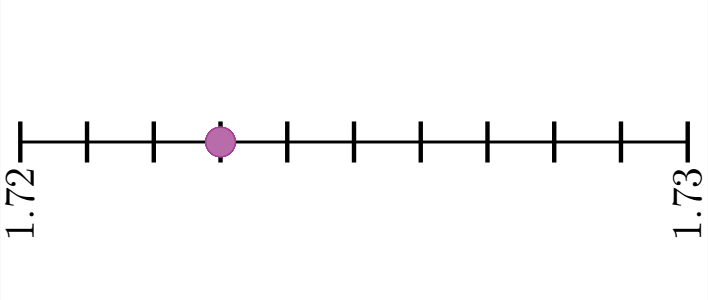
\includegraphics[width=0.7\linewidth]{../images/recta_num_1.723.png}\\[-0.5em]  \fillin[$1.723$][1.5in]
				
				% \part 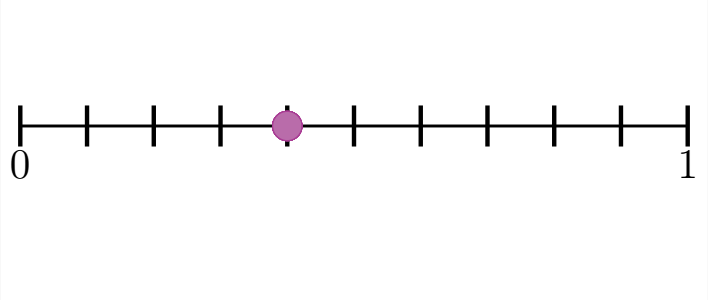
\includegraphics[width=0.7\linewidth]{../images/recta_num_0.4.png}  \\[-0.5em]  \fillin[$0.4.$][1.5in]
				
				% \part 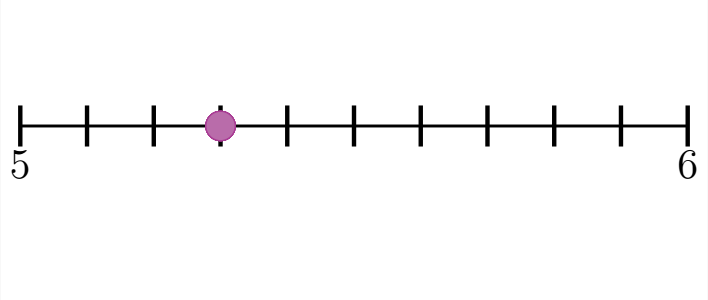
\includegraphics[width=0.7\linewidth]{../images/recta_num_5.3.png}  \\[-0.5em]  \fillin[$5.3.$][1.5in]
				
				% \part 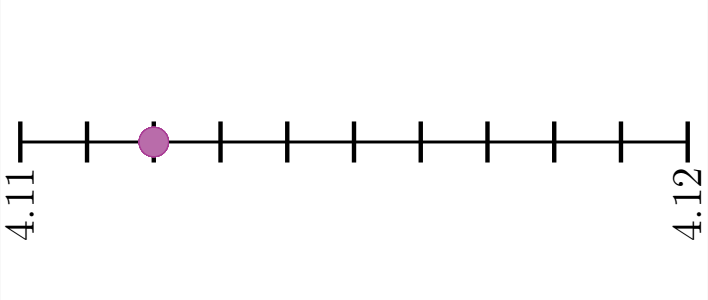
\includegraphics[width=0.7\linewidth]{../images/recta_num_4.112.png}\\[-0.5em]  \fillin[$4.11$][1.5in]
				
				% \part 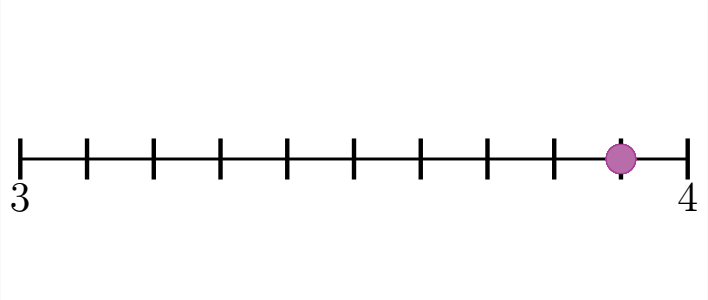
\includegraphics[width=0.7\linewidth]{../images/recta_num_3.9.png}  \\[-0.5em]  \fillin[$3.9.$][1.5in]
			\end{parts}
		\end{multicols}